\begin{figure}[H]
\label{fig-beamtransformed}
\caption{The effective cross-section of the beam (all dimensions in mm)}
\centering
\vspace{1em}
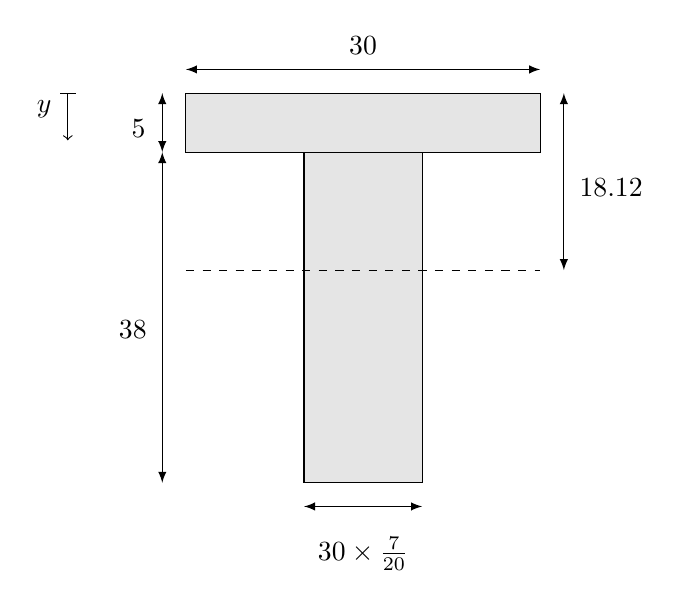
\begin{tikzpicture}[scale=0.3]
    \draw[|-to] (-5, 0) -- (-5,-2);
    \node[] at (-6, -0.7) {$y$};
    \draw[latex-latex] (0,1) -- (15,1);
    \draw[latex-latex] (-1,0) -- (-1, -2.5);
    \draw[latex-latex] (-1,-2.5) -- (-1, -16.5);
    \draw[latex-latex] (5,-17.5) -- (10, -17.5);
    \draw[latex-latex] (16,0) -- (16,-7.5);
    \draw[draw=black, fill=gray!20] (0,0) rectangle (15,-2.5);
    \draw[draw=black, fill=gray!20] (5,-2.5) rectangle (10,-16.5);
    \node[] at (7.5, 2) {30};
    \node[] at (7.5, -19.5) {$30 \times \frac{7}{20}$};
    \node[] at (-2, -1.5) {5};
    \node[] at (-2.25, -10) {38};
    \node[] at (18,-4) {18.12};
    \draw[dashed] (0,-7.5) -- (15,-7.5);
\end{tikzpicture}
\end{figure}
    